% !TeX program = xelatex
% !TeX encoding = utf-8
% 《机器人》LaTeX模板
% 面向往复夹持递送的血管介入机器人力反馈扰动建模与残差补偿

% 仅指定文档类路径，避免读入模板目录内其他稿件的编译缓存。
\documentclass{JQR_LaTeX_Template-0507/JQRnew}


% 修订标记：正文及公式按原稿逐段对照；干净版关闭颜色。
\providecommand{\RevisionColor}{\color{black}}
\newcommand{\revised}[1]{{\RevisionColor#1}}
\newcommand{\revbegin}{\begingroup\RevisionColor}
\newcommand{\revend}{\par\endgroup}

\JQRsetup{
 % 期刊出版信息
 volume     = xx,
 number     = x,
 year       = 2026,
 month      = 10,
 doi        = 240001,
 % 通信作者
 corrauthor = {\revised{胡琨元（Email：[待补]）；刘浩，Email: liuhao@sia.cn}},
 % 日期
 dates      = {2026-10-21/2026-10-21/2026-10-21},
 %
 % ---- 中文相关信息
 cntitle    = {面向往复夹持递送的血管介入机器人力反馈扰动建模与残差补偿},
 cnauthor   = {隋凯丞\addr{1,2,3}, 郑力铭\addr{1,2,3}, 林\quad 鹏\addr{1,2}, 胡琨元\addr{1,2*}, 刘\quad 浩\addr{1,2*}},
 runtitle   = {隋凯丞，等：面向往复夹持递送的血管介入机器人力反馈扰动建模与残差补偿},
 cnaddress  = {1. 中国科学院沈阳自动化研究所 机器人学国家重点实验室，辽宁~~沈阳\quad 110016；\\
               2. 辽宁省微创手术机器人重点实验室，辽宁~~沈阳\quad 110016；\\
               3. 中国科学院大学，北京\quad 100049},
 %
 % ----- 中文摘要
cnabstract = {\revbegin
针对夹持式血管介入机器人往复夹持递送引起的近端测力波动，建立轴向力反馈重构方法。按递送、承载切换和重新承载过程划分往复周期，校正测量信号中的空载响应项。以前向推进行程为自变量，将重新推进时的轴向载荷恢复描述为传力链弹性加载与停顿后附加摩擦阻力衰减的共同作用，建立轴向载荷恢复模型。以切换时确定的载荷量、机构运动和推进行程为输入，采用门控循环单元（GRU）提取单周期恢复过程的时序特征。跨周期注意力机制聚合前序周期相同行程位置的特征，估计物理模型未描述的残差，网络输入不包含恢复阶段的实时测力。多数测试周期的恢复曲线出现局部峰值。计入停顿后附加摩擦阻力后，恢复模型能够描述局部峰值和起步段载荷变化。离线叠加阻力测试中，本文方法完整保留了重新承载后推进期间新增阻力的变化。反馈重构误差及操作者实验结果为[待补]。所建方法结合物理模型和跨周期残差估计，实现往复夹持递送中的轴向力反馈重构。
\revend},
 % ---- 中文关键字
 cnkeywords = {\revised{介入机器人；往复夹持；轴向力反馈；载荷恢复；门控循环单元；跨周期注意力}},
 %
 % ---- 英文相关信息
 entitle    = {Disturbance Modeling and Residual Compensation of Force Feedback for Vascular Intervention Robot in Reciprocating Clamping Delivery},
 enauthor   = {\revised{SUI Kaicheng\addr{1,2,3}, ZHENG Liming\addr{1,2,3}, LIN Peng\addr{1,2}, HU Kunyuan\addr{1,2*}, LIU Hao\addr{1,2*}}},
 enaddress  = {1. \textit{State Key Laboratory of Robotics, Shenyang Institute of Automation, Chinese Academy of Sciences, Shenyang} 110016, \textit{China}; \\
               2. \textit{Key Laboratory of Minimally Invasive Surgical Robot, Liaoning Province, Shenyang} 110016, \textit{China}; \\
               3. \textit{University of Chinese Academy of Sciences, Beijing} 100049, \textit{China}},
 %
 % ---- 英文摘要
 enabstract = {\revbegin
[Objective] To develop an axial force feedback reconstruction method for proximal measurement fluctuations caused by reciprocating clamping delivery in a vascular intervention robot. [Methods] The reciprocating cycle is divided into delivery, load transfer, and reloading phases, and the zero-load response term in the measured signal is corrected. Using forward travel as the independent variable, an axial load recovery model combines elastic loading of the force transmission chain with decay of additional frictional resistance after a hold. A gated recurrent unit (GRU) encodes each recovery process using load quantities determined at the transition, mechanism motion, and forward travel. Cross-cycle attention aggregates features at corresponding travel positions in preceding cycles to estimate residuals not described by the physical model. Network inputs exclude real-time force measurements during recovery. [Results] Local peaks occurred in the recovery curves of most test cycles. When additional frictional resistance after a hold was included, the recovery model described local peaks and initial load changes. In offline resistance superposition tests, the proposed method fully preserved the added resistance during forward delivery after reloading. Feedback reconstruction errors and operator-task results are [待补]. [Conclusions] The method combines physical modeling and cross-cycle residual estimation to reconstruct axial force feedback during reciprocating clamping delivery.
\revend},
 %
 % ---- 英文关键字
 enkeywords = {\revised{intervention robot; reciprocating clamping; axial force feedback; load recovery; gated recurrent unit (GRU); cross-cycle attention}}
}

% ----- 加载宏包
\usepackage{algorithm}
\usepackage{algpseudocode}
\usepackage{pifont}
\usepackage{balance}
\usepackage{mwe}
\usepackage{booktabs}
\usepackage{amsmath,amssymb}
\usepackage{bm}
\usepackage{enumitem}
\usepackage{float}
\graphicspath{{JQR_LaTeX_Template-0507/}}
% 修订稿用 draft；干净稿改为 final。中文删除线支持自动换行。
\usepackage[draft,commentmarkup=footnote]{changes}
\usepackage{xeCJKfntef}
\setdeletedmarkup{\CJKsout{#1}}

\floatname{algorithm}{算法}
\renewcommand{\algorithmicrequire}{\textbf{输入:}}
\renewcommand{\algorithmicensure}{\textbf{输出:}}
\newcommand{\algorithmicchushi}{\textbf{初始化:}}

\begin{document}

\maketitle
% 栏底留白，避免通栏图下方正文被拉伸以强制对齐两栏底部。
\raggedbottom

% 引言部分不设节标题（遵循《机器人》期刊约定）
% 首栏由模板预留页脚空间，换栏时为第二栏预留相同高度。
\makeatletter
\AddToHookNext{cmd/@outputdblcol/after}{\JQRpubidadjcol}
\makeatother
血管介入机器人通过主从遥操作驱动导丝和导管完成推进与旋转，使术者能够免遭X射线辐射伤害\ucite{ref2}。在手动递送中，术者通过指端感受器械阻力，并结合影像判断器械的运动与受力状态，但在遥操作中，这种触觉联系需要通过从端测量和主端力反馈重建，接触力的测量很大程度影响着术者的认知，并进一步影响着手术的安全性\ucite{ref29}。力反馈既需要反映器械与环境之间的相互作用，也需要减少不必要的干扰波动，使术者能够辨别操作阻力的变化。

 从测量位置看，血管介入机器人相关的力感知可分为体内远端测力和体外近端测力。远端方案将微型传感元件集成于器械尖端，以获取局部接触载荷。例如，He等\ucite{ref3}在导管尖端集成光纤布拉格光栅传感器，测量导管与血管壁之间的接触力；Kesner和Howe\ucite{ref34}将光纤测力元件与消融电极集成于导管末端，结合超声引导实现导管与运动组织之间的接触力控制；Jin等\ucite{ref35}在导管尖端设置自研力传感器，测量导管尖端与血管壁之间的碰撞力，并结合导丝和导管的受力分析提高力反馈信息的可用性。这类方案需要兼顾器械尺寸、传感元件封装、弯曲性能与生物相容性，传感器集成也增加了器械制造与临床适配的复杂性。

 近端测力的一类实现方式是根据驱动电机电流建立载荷估计。Sankaran等\ucite{ref5}根据驱动电机的电流和转速标定空载运行偏置，以估计滚轮驱动器械时的近端操作力。电流信号同时受到电机参数、传动摩擦、机构惯性和夹持状态的影响，电流与器械载荷之间的映射依赖具体机构和运行工况的标定，难以直接区分器械外载与机构自身运动引起的载荷。另一类实现方式是在器械夹持或传动路径中设置负载传感器，使器械载荷经夹持件、滑动件或弹性传力构件传递至测量元件。Zhao等\ucite{ref4}将负载传感器集成于滑动机构，测量导丝和导管的轴向操作力，并通过弹性结构上的应变传感器测量旋转载荷；Wang等\ucite{ref12}将轴向力和旋转力矩测量功能集成于介入机器人机构中；Jin等\ucite{ref36}在从端夹持结构中设置负载传感器，分别测量导丝和导管的轴向力，并配合扭矩传感器实现力反馈。此类布置保留了常规介入器械的末端结构，但测量结果取决于器械载荷、夹持状态以及机构内部传力路径的共同作用。

  滚轮式机构通过相向压紧的滚轮与器械之间的摩擦传递驱动力，滚轮连续转动即可实现长距离推进。Thakur等\ucite{ref37}采用高摩擦驱动轮、弹簧加载从动滚轮和附加滚轮组保持导管与驱动轮接触，实现导管的连续轴向推进；Sankaran等\ucite{ref5}在滚轮驱动系统中利用驱动电机电流估计近端操作力，并通过空载电流与转速之间的关系标定运行偏置；Chowdhury等\ucite{ref38}提出双主动倾斜滚轮驱动机构，在同一模块中实现器械平移与旋转，并通过调整滚轮位置适配不同直径的介入器械。此类机构具有连续递送和结构紧凑等特点，但其驱动力受到接触摩擦和压紧程度的限制，压紧不足时易发生相对滑移，增大压紧力则会提高器械局部受压变形及表面损伤的风险。

  仿生手指夹持机构通过相对设置的夹持面夹紧器械，利用夹持接触产生的摩擦传递轴向和旋转载荷。夹持机构可安装于直线运动平台完成轴向平移，并通过旋转单元带动器械绕轴转动，平移与旋转分别驱动和控制\ucite{ref6,ref15}。Wang等设计了多夹持器血管介入机器人，将夹持递送与轴向、旋转力反馈结合\ucite{ref6}；针对有限行程造成的连续递送问题，Wang等提出由夹持、推进、释放和回程组成的往复操作方法\ucite{ref9}，Cao等进一步将往复递送装置与多操作器协同，用于导丝和导管的配合操作\ucite{ref10}。Al-Ahmad等采用编织套夹持器，通过双夹持器的交替夹持和重叠承载实现介入器械的连续运动\ucite{ref7}。在带测力功能的夹持结构中，传感器通常布置在夹持组件与驱动支撑件之间，使器械载荷沿夹持传力路径传递至测量元件；在往复递送结构中，递送机构与支撑机构交替完成夹持、推进、释放和回程，使器械载荷的传递路径随动作阶段发生改变。

\revbegin
递送机构与支撑机构交替夹持，使递送机构的轴向测力通道在每个往复周期内经历承载、卸载和重新承载。在递送机构的夹持组件内集成传感器的结构中，器械外载经夹持组件传至传感器；当支撑机构接替承载、递送机构的夹持组件松开时，原测力通道随之卸载。递送机构回程及重新夹持伴随姿态变化和夹持组件开合冲击，旋转姿态相关的空载响应和夹持动作瞬态叠加在测量信号中。近端信号的变化既包含器械阻力变化，也包含承载切换、载荷松弛与恢复引起的变化。将这些变化直接反馈至主端，会造成与递送动作同步的力觉波动，影响术者对器械受力状态的判断。
\revend

 针对机构运动和传力过程对力感知的影响，已有研究从运动附加载荷校正与传力过程建模两方面开展分析。运动补偿通过测力部件的受力分析，建立与载荷、旋转速度相关的补偿关系\ucite{ref8}，或结合平移与旋转动力学、夹紧与松开状态下的对比测量及滤波，减小机构运行引起的测量误差\ucite{ref12}。在接触与柔性传动建模中，黏弹性接触模型和动态摩擦模型分别描述接触载荷的时间变化与摩擦过渡过程\ucite{ref20,ref28}；腱鞘模型则将路径构型、输入张力与受力伸长联系起来，用于传动偏差的分析与补偿\ucite{ref30}。这些研究为校正运动附加载荷和描述柔性传力过程提供了依据。然而，往复夹持递送中的周期性承载切换使测力通道反复卸载和重新承载，器械不断深入又改变了接触位置与载荷分布。按固定工况建立的低阶动力学模型难以同时描述这些阶段变化与跨周期偏差，补偿过程还需保留真实操作阻力的变化。
\revbegin
针对上述问题，本文提出结合物理建模与残差学习的轴向力反馈重构方法，分析承载切换引起的测量变化。以弹性加载与停顿后附加摩擦阻力衰减描述重新推进时的轴向载荷恢复，采用GRU及跨周期注意力估计物理模型未描述的残差，并在自主研制的血管介入机器人上开展血管模型递送实验。
\revend



\section{问题描述（Problem description）}

\subsection{往复夹持递送过程}

\revbegin
本文研究的夹持式血管介入机器人采用递送机构（M）和支撑机构（S）交替夹持器械，通过夹持组件与器械表面的摩擦接触传递运动和载荷。递送机构安装于沿直线导轨移动的滑台上，负责器械的轴向推进与周向旋转，其夹持组件内集成轴向与周向两路测力通道；支撑机构安装于近血管鞘入口端，在递送机构释放与回退期间保持器械位置。
\revend

\revbegin
受直线导轨行程限制，长距离递送由周期性短行程往复运动完成。根据运动和夹持时序，将一个往复周期划分为S1～S10十个阶段，如图\ref{fig1}所示。
\begin{figure}[!b]
\RevisionColor
\centering
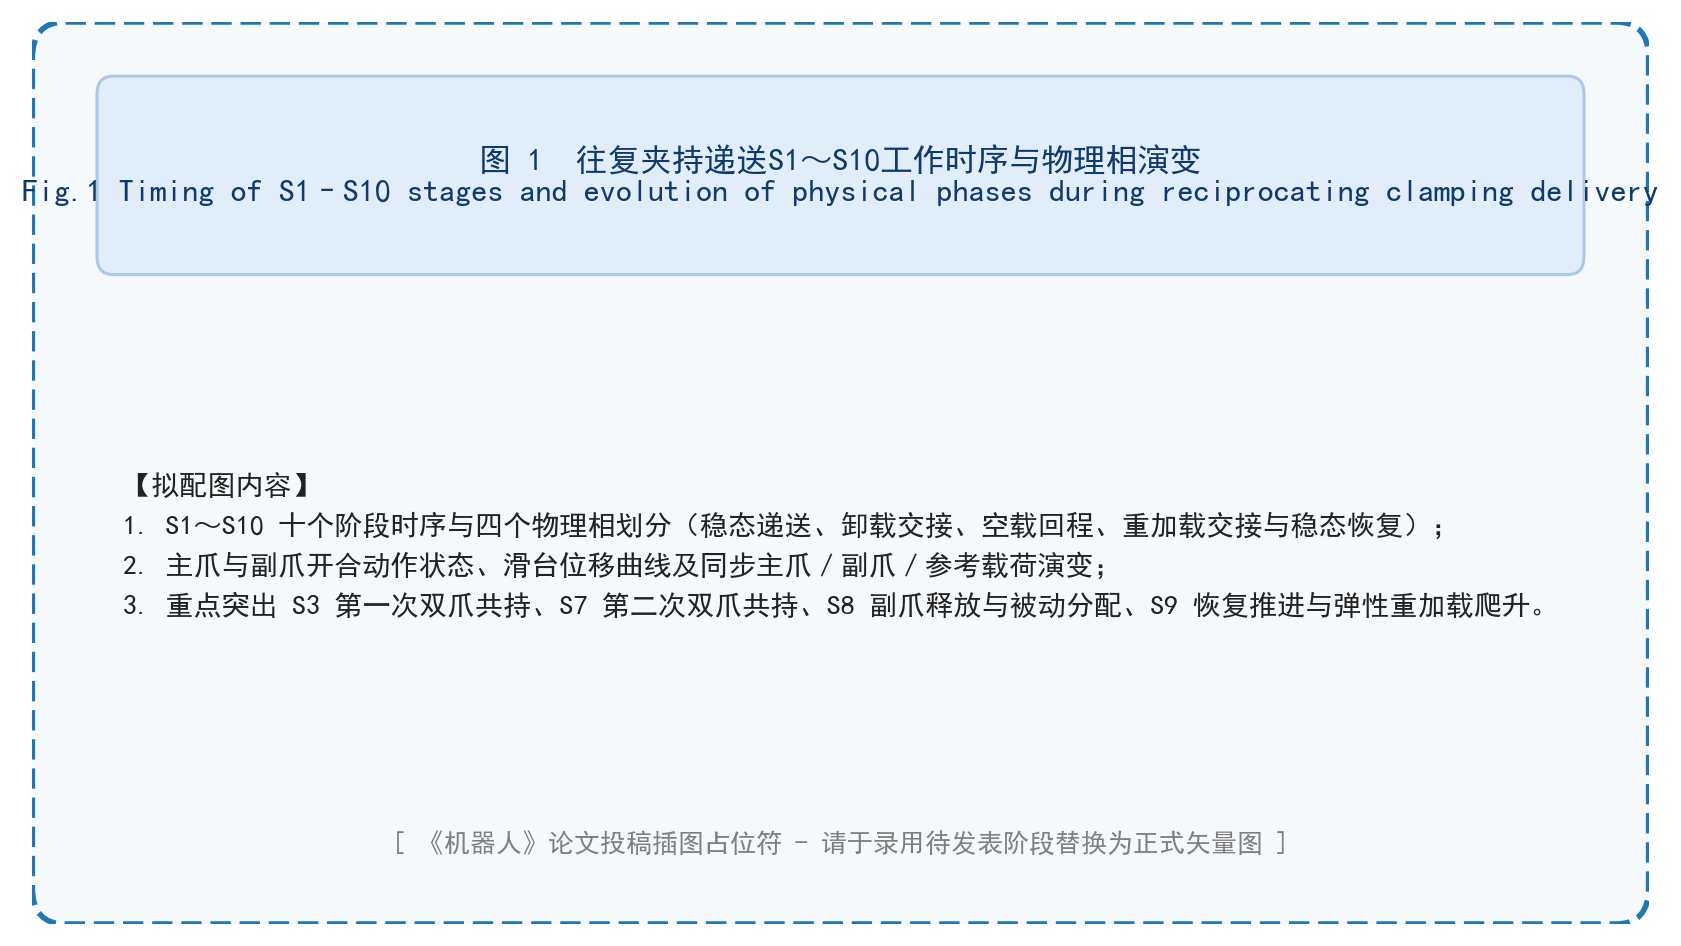
\includegraphics[width=\linewidth]{fig1.png}
\bicaption{\revised{往复夹持递送工作过程}}{\revised{Stages of reciprocating clamping delivery}}
\label{fig1}
\end{figure}
\begin{enumerate}[label=\arabic*),nosep,itemsep=0pt,topsep=2pt,partopsep=0pt,parsep=0pt,leftmargin=2\ccwd]
\item 递送与停止（S1～S2）：递送机构独立夹持器械推进，并可同时旋转（S1）；单次行程结束时滑台减速停止，支撑机构尚未闭合（S2）。
\item 承载切换（S3～S4）：支撑机构闭合，两个机构共同夹持器械（S3）；随后递送机构释放，由支撑机构承载（S4）。
\item 空载回程（S5～S6）：递送机构脱离器械后沿导轨退回（S5），在起点减速停止（S6），期间器械由支撑机构保持。
\item 重新承载与递送（S7～S10）：递送机构在起点闭合，两个机构再次共同夹持（S7）；支撑机构释放后，静止的递送机构独立承载（S8）；递送机构恢复前向推进，在规定行程窗口内补偿重新承载时的载荷变化（S9）；补偿撤除后进入正常递送阶段（S10）。
\end{enumerate}
\revend

\subsection{测力波动与补偿目标}

\revbegin
往复夹持递送使轴向测力通道周期性经历承载、卸载和重新承载。空载响应随旋转姿态变化；夹持组件开合冲击、停止后的载荷松弛及重新推进时的载荷恢复也会反映在近端测量信号中。
\revend

本文以连续递送时的器械载荷作为反馈目标，参考载荷取匹配插入位置与运动条件的连续递送实测力（2.1节）。在S1末锁存轴向稳态载荷，S2～S8保持该值；S9以前向推进行程描述轴向载荷恢复，并由两级残差估计网络修正恢复模型的残差；轴向输出由校正测量值与补偿量相加得到。扭矩通道只进行测量校正和S2～S8输出保持，S9起输出校正测量值。

\revbegin
全文设轴向正方向沿器械名义中心轴指向远端，旋转角正方向遵循右手定则。力、扭矩、位移、角位移和时间的单位分别为 $\mathrm{N}$、$\mathrm{N}\cdot\mathrm{mm}$、$\mathrm{mm}$、$\mathrm{rad}$ 和 $\mathrm{s}$。轴向传感器读数记为 $F_{xm}$，周向测力通道的切向力读数记为 $F_{tm}$，经标定等效力臂 $\ell_s$ 换算得到测量扭矩 $\tau_{xm}=\ell_sF_{tm}$。输出至主端的反馈信号统一记为 $\bm w_{\mathrm{fb}}=[F_{\mathrm{fb}},\tau_{\mathrm{fb}}]^{\rm T}$。
\revend

\subsection{本文工作}

本文围绕往复夹持递送中的轴向力反馈重构开展以下工作。
\begin{enumerate}[label=\arabic*),nosep,itemsep=0pt,topsep=2pt,partopsep=0pt,parsep=0pt,leftmargin=2\ccwd]
\item 建立测量干扰模型和递送机构与支撑机构的受力关系，以S1末稳态载荷和S8末实测载荷确定轴向载荷恢复补偿的初值。
\item \revbegin 建立基于弹性加载与停顿后附加摩擦阻力衰减的轴向载荷恢复模型。结合两级残差估计网络修正、切换期间的输出保持和补偿量平滑撤除，形成分阶段反馈方法。\revend
\item \revbegin 通过参数辨识、参考误差分析、叠加阻力测试和消融比较评价轴向力重构，并在血管模型中比较介入总时间和通过成功率。\revend
\end{enumerate}

\revbegin
第2节介绍受力关系、轴向载荷恢复模型与反馈方法，第3节给出实验配置和评价方法，第4节与第5节分别为讨论和结论。
\revend

\section{往复夹持传力与反馈补偿方法（Load transmission and feedback compensation for reciprocating clamping）}

\subsection{测量关系、递送机构与支撑机构的受力及参考载荷}

\revbegin
递送机构的测力通道与递送机构、支撑机构的受力关系如图\ref{fig2}所示。两机构之间的器械段不与其他物体接触，支撑机构远端的鞘管和血管壁对器械的作用计入外载。忽略器械自身惯性，轴向力和绕轴扭矩满足
\revend
\begin{equation}
\label{eq:balance}
\begin{cases}
F_M+F_S=F_{\mathrm{out}},\\
\tau_M+\tau_S=\tau_{\mathrm{out}}.
\end{cases}
\end{equation}
式中，$F_M,\tau_M$ 与 $F_S,\tau_S$ 分别为递送机构和支撑机构作用于器械的轴向推力和驱动扭矩，以向远端推进和按右手定则正转为正；$F_{\mathrm{out}},\tau_{\mathrm{out}}$ 为外部轴向合阻力和合阻力矩，以阻碍上述正向运动为正。记 $\bm w_M=[F_M,\tau_M]^{\rm T}$。支撑机构完全释放时 $F_S=\tau_S=0$，外载全部由递送机构平衡。

\revbegin
将轴向力与换算后的扭矩组成测量向量 $\bm y=[F_{xm},\ell_sF_{tm}]^{\rm T}$。传感器连接浮动传力组件与滑台。测力传感器前侧的浮动传力组件质量较小，血管介入递送速度为 $\mathrm{cm/s}$ 量级，启停引起的惯性力低于传感器分辨率，测量关系中不计入惯性项。测量关系写为
\begin{equation}
\label{eq:measurement}
\bm y=\bm H_0\bm w_M+\bm b(\varphi_M)+\bm p_{\mathrm{clamp}}(t)+\bm\varepsilon.
\end{equation}
式中，$\bm q_M=[x_M,\dot x_M,a_M,\varphi_M,\dot\varphi_M,\alpha_M]^{\rm T}$ 为平移轴和旋转轴的位置、速度及加速度向量；$\bm H_0\in\mathbb R^{2\times2}$ 为离线标定的可逆传递矩阵，非对角元包含力与扭矩之间的单位换算；$\bm b(\varphi_M)$ 为空载响应项，包含静态零偏和随旋转角变化的重力分量；$\bm\varepsilon$ 为测量噪声。各向量的两个分量依次以 $\mathrm{N}$ 和 $\mathrm{N}\cdot\mathrm{mm}$ 计。
\revend

\revbegin
开合指令记为 $\bm c=[c_M,c_S]^{\rm T}\in\{0,1\}^2$，闭合取1、释放取0。$\bm p_{\mathrm{clamp}}(t)$ 为夹持组件开合引起的短时冲击。开合动作发生在S3、S4、S7和S8，这些阶段的反馈采用输出保持值。扣除空载响应项后的校正测量值为
\begin{equation}
\label{eq:corrected-measurement}
\bm w_{\mathrm{meas}}[k]=\bm H_0^{-1}\!\left[
\bm y[k]-\bm b(\varphi_M[k])\right].
\end{equation}
\revend

单机构递送阶段（S1、S9、S10）支撑机构完全释放，递送机构独自平衡外载。S3～S7中支撑机构参与或独自承载（$F_S\neq0$），递送机构的测力通道在S4～S6卸载，并在S7原位重新闭合。由于夹持面与传力链存在柔顺性，S7递送机构刚闭合时尚未形成明显的切向变形，外载仍主要由支撑机构承担，此时递送机构的测量值不反映外载。S8支撑机构释放后，静止的递送机构重新独自承载；承载切换过程中传力链的部分变形已经释放，S8末递送机构实测载荷低于切换前的稳态值。取S8末支撑机构释放冲击衰减后、平移轴与旋转轴均静止（$a_M=\alpha_M=0$）的采样时刻 $k_9$，递送机构承载的初值为
\begin{equation}
\label{eq:initial-load}
\widehat{\bm w}_{M,k_9}
=\bm H_0^{-1}\!\left[\bm y[k_9]-\bm b(\varphi_M[k_9])\right].
\end{equation}

反馈的目标是连续递送时的器械载荷。参考载荷取同一器械、鞘管和模型路径下，匹配插入位置与运动条件的连续递送实测力。配对试次采用一致的起始插入状态，在有效递送区间匹配平移与旋转的速度、加速度及运动方向。以累计有效插入深度 $s$ 为自变量，参考载荷定义为
\begin{equation}
\label{eq:reference}
\bm w_{\mathrm{ref}}(s[k])
=\bm w_{\mathrm{meas}}^{\mathrm{cont}}(s[k]).
\end{equation}
式中，$\bm w_{\mathrm{meas}}^{\mathrm{cont}}$ 为配对连续递送记录的校正测量值，两个分量分别为轴向力与扭矩。S2减速推进的位移计入 $s$，递送机构空载回程不计入；器械保持同一插入位置时，参考值保持为连续记录中该位置的值。参考数据用于网络监督和离线评价，不参与在线补偿计算。配对方法见3.1节。

\begin{figure}[H]
\centering
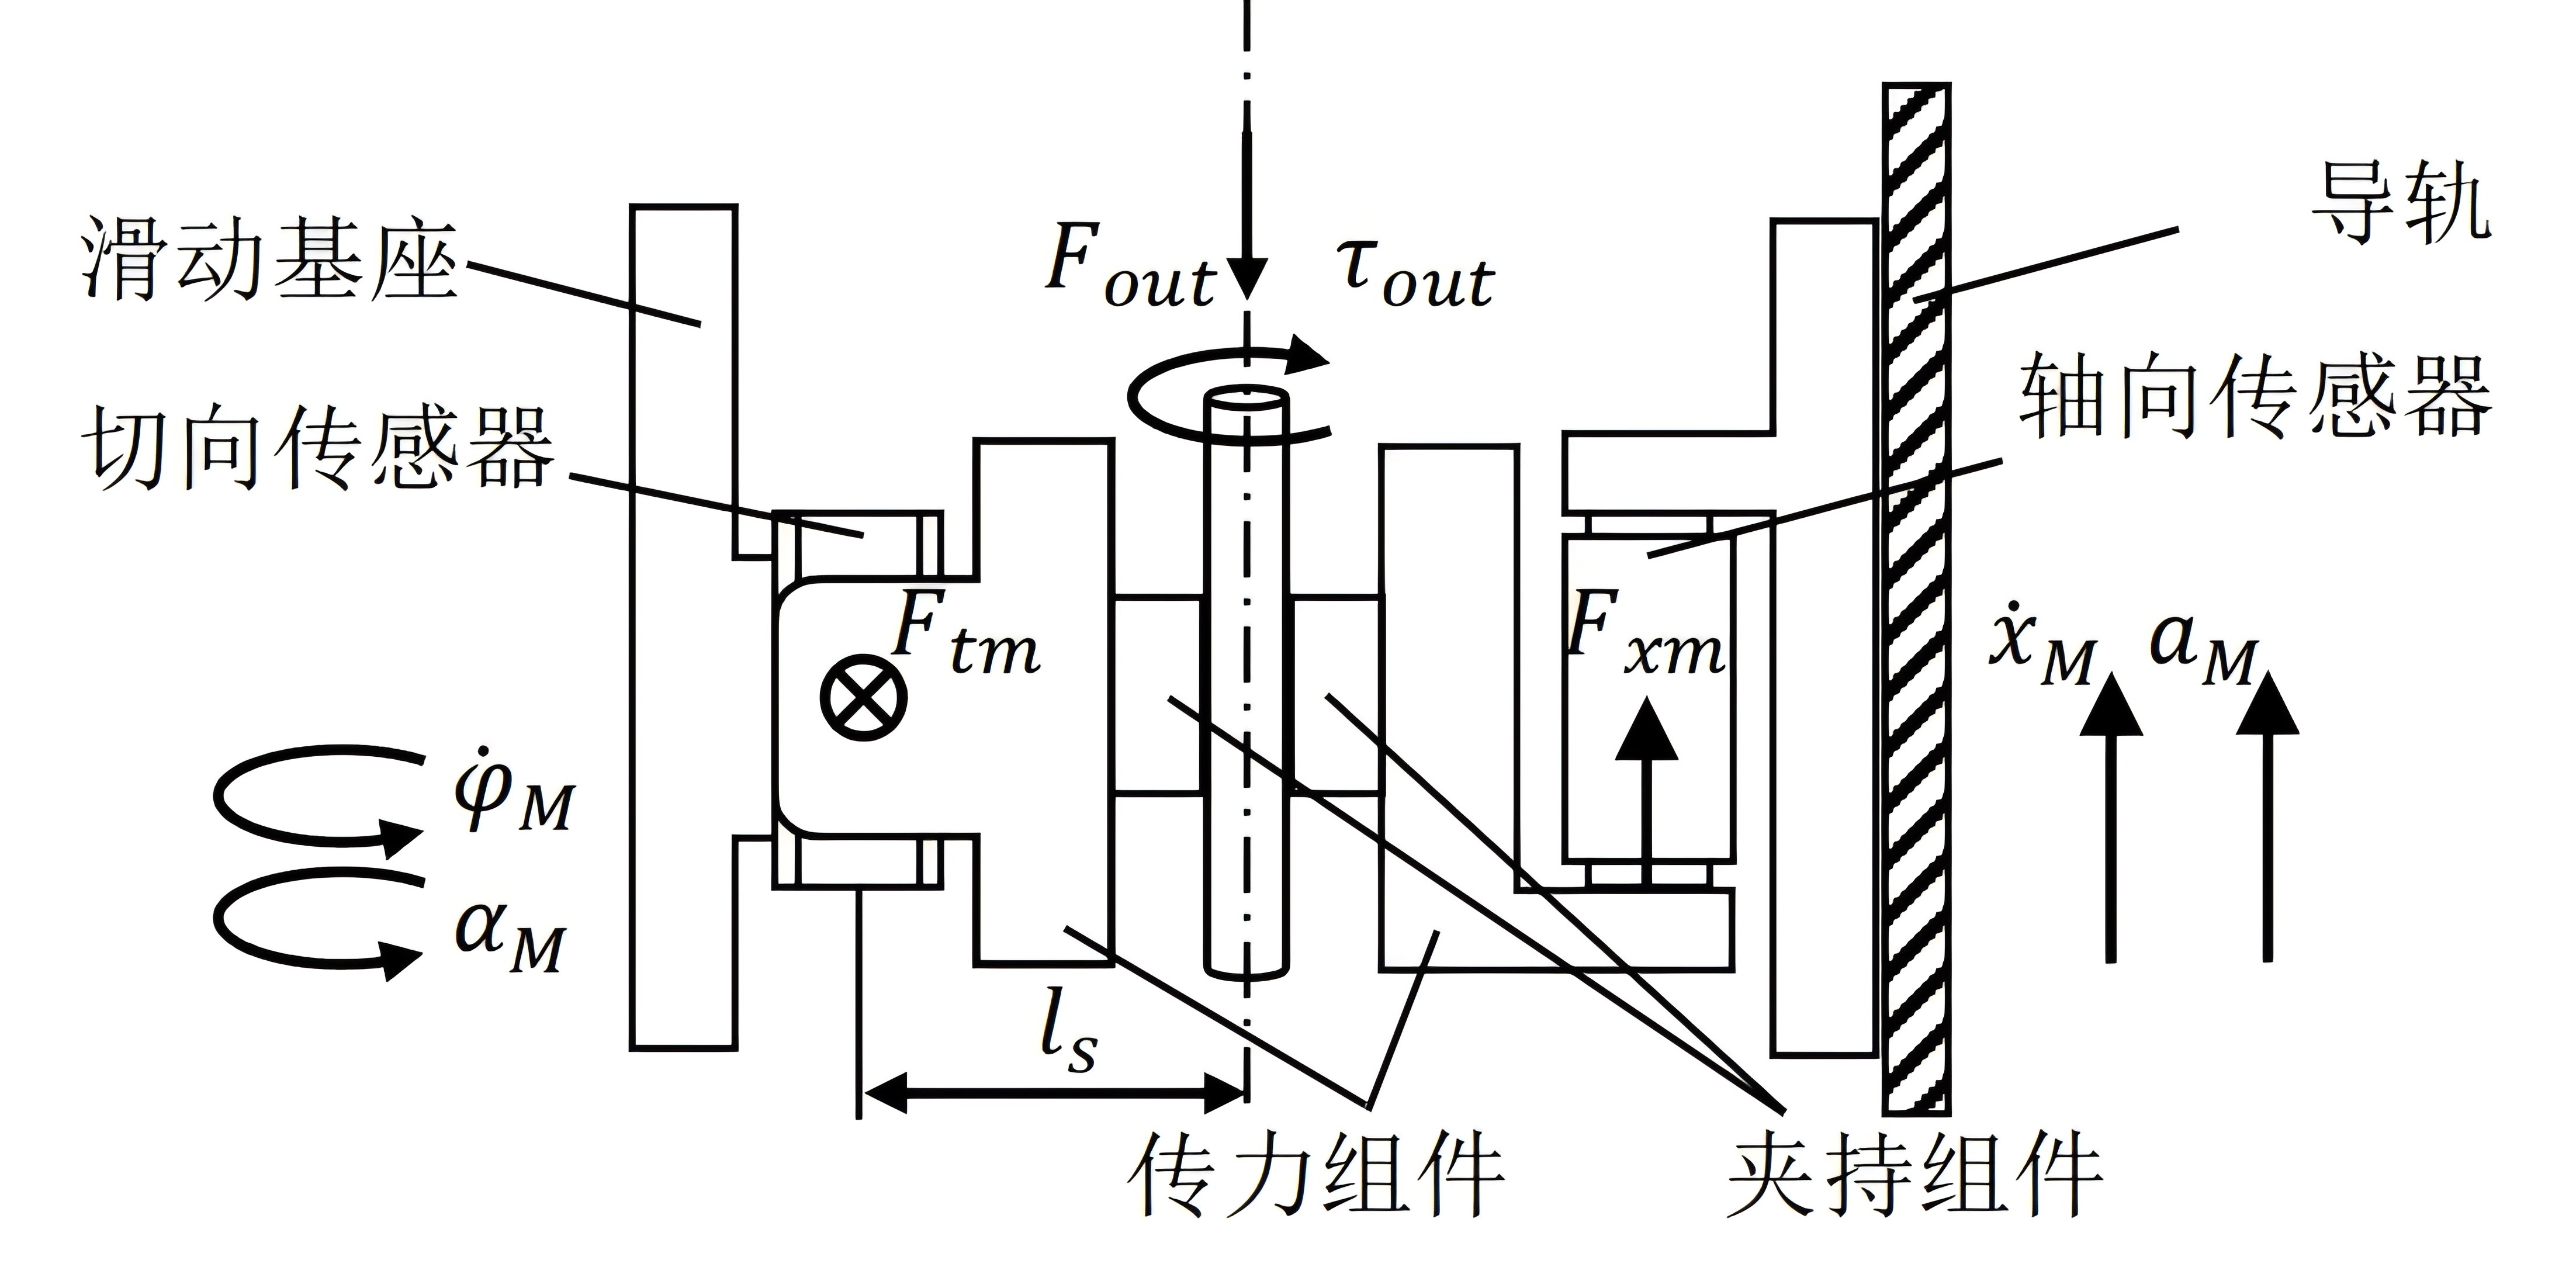
\includegraphics[width=\linewidth]{./figure2_manuscript.png}
\bicaption{测力通道与递送机构、支撑机构的受力关系}{Force-sensing channels and load transfer between the delivery and support mechanisms}
\label{fig2}
\end{figure}

\subsection{重新承载后的轴向载荷恢复模型}

S1匀速段末的切换前稳态载荷向量记为
\begin{equation}
\label{eq:lock}
\widehat{\bm D}_9=\frac{1}{N_{\mathrm{lock}}}
\sum_{j=k_{\mathrm{S1,end}}-N_{\mathrm{lock}}+1}^{k_{\mathrm{S1,end}}}
\bm w_{\mathrm{meas}}[j].
\end{equation}
式中，$k_{\mathrm{S1,end}}$ 为减速指令发出前的最后一个采样时刻，$N_{\mathrm{lock}}$ 为完全位于匀速段内的窗口长度。切换前后的轴向载荷差定义为待恢复载荷差：
\begin{equation}
\label{eq:deficit}
\widehat A_{9,F}=\widehat D_{9,F}-\widehat w_{M,k_9,F}.
\end{equation}

恢复模型用于 $\widehat A_{9,F}>0$ 的前向推进过程。自S8末起累计前向推进行程
\begin{equation}
\label{eq:recovery-travel}
s_{\mathrm{rec}}(t)=\int_{t_{\mathrm{S8,end}}}^{t}
\max\!\left(\dot x_M(t'),0\right)\,\mathrm dt'.
\end{equation}
\revbegin
S9中的轴向载荷恢复包含两部分作用。一是递送机构重新承载后，夹持组件、浮动传力组件及器械段组成的串联传力链随推进逐步加载。二是器械在S2～S8静止后，与鞘管和血管壁之间的静摩擦大于滑动摩擦，重新推进时形成附加阻力，并在一定滑移距离内过渡至滑动摩擦水平\cite{dahl1968,ruina1983}。S8静止期间载荷不随时间回升，恢复只在前向推进时发生，因此以推进行程为自变量。令 $w_F(s_{\mathrm{rec}})$ 为模型给出的轴向载荷，采用一阶恢复关系
\revend
\begin{equation}
\label{eq:recovery-ode}
\frac{\mathrm dw_F}{\mathrm ds_{\mathrm{rec}}}
=\frac{\widehat D_{9,F}+\Delta_F e^{-s_{\mathrm{rec}}/D_c}-w_F}{\lambda_F}.
\end{equation}
\revbegin
式中，$\lambda_F>0$ 为弹性加载的特征行程，$\Delta_F\ge0$ 为停顿后附加摩擦阻力的幅值，$D_c>0$ 为附加阻力衰减的特征滑移距离。三个参数由辨识集的恢复曲线离线联合确定，在各周期的在线补偿中保持不变。以 $w_F(0)=\widehat w_{M,k_9,F}$ 为初值积分，得到相对于切换前载荷的补偿量
\revend
\begin{equation}
\label{eq:recovery-comp}
\begin{aligned}
f_{\mathrm{rel},F}(s_{\mathrm{rec}})&=\widehat D_{9,F}-w_F(s_{\mathrm{rec}})\\
&=\widehat A_{9,F}e^{-s_{\mathrm{rec}}/\lambda_F}\\
&\quad-\frac{\Delta_FD_c}{D_c-\lambda_F}
\left(e^{-s_{\mathrm{rec}}/D_c}-e^{-s_{\mathrm{rec}}/\lambda_F}\right).
\end{aligned}
\end{equation}
当 $D_c=\lambda_F$ 时，取极限形式
\begin{equation}
\label{eq:equal-scales}
f_{\mathrm{rel},F}(s_{\mathrm{rec}})=
\left(\widehat A_{9,F}-\Delta_F\frac{s_{\mathrm{rec}}}{\lambda_F}\right)e^{-s_{\mathrm{rec}}/\lambda_F}.
\end{equation}
\revbegin
当 $\Delta_F=0$ 时，只剩弹性加载项，载荷单调趋近切换前载荷。若不计弹性加载项（$\lambda_F\to0$），载荷在重新推进起点即跳回切换前载荷附近，与S8末实测的待恢复载荷差不符。若恢复曲线出现高于切换前载荷的局部峰值，$f_{\mathrm{rel},F}$ 在局部峰值附近为负，即从实测值中扣除附加阻力分量。
\revend

令式\eqref{eq:recovery-ode}右端为零，得到局部峰值对应的行程
\begin{equation}
\label{eq:peak-location}
\begin{aligned}
s^*&=\frac{\lambda_FD_c}{D_c-\lambda_F}
\ln\frac{(\widehat A_{9,F}+B)D_c}{B\lambda_F},\\
B&=\frac{\Delta_FD_c}{D_c-\lambda_F}.
\end{aligned}
\end{equation}
\revbegin
对于 $\widehat A_{9,F}>0$、$\Delta_F>0$，$D_c>\lambda_F$ 时存在位于有限行程内的局部峰值；$D_c<\lambda_F$ 时还需满足 $\widehat A_{9,F}<\Delta_FD_c/(\lambda_F-D_c)$。两尺度相等时，$s^*=\lambda_F(1+\widehat A_{9,F}/\Delta_F)$；$\Delta_F=0$ 时载荷单调趋近参考值。
\revend
恢复过程及补偿量如图\ref{fig3}所示。

\begin{figure}[!t]
\centering
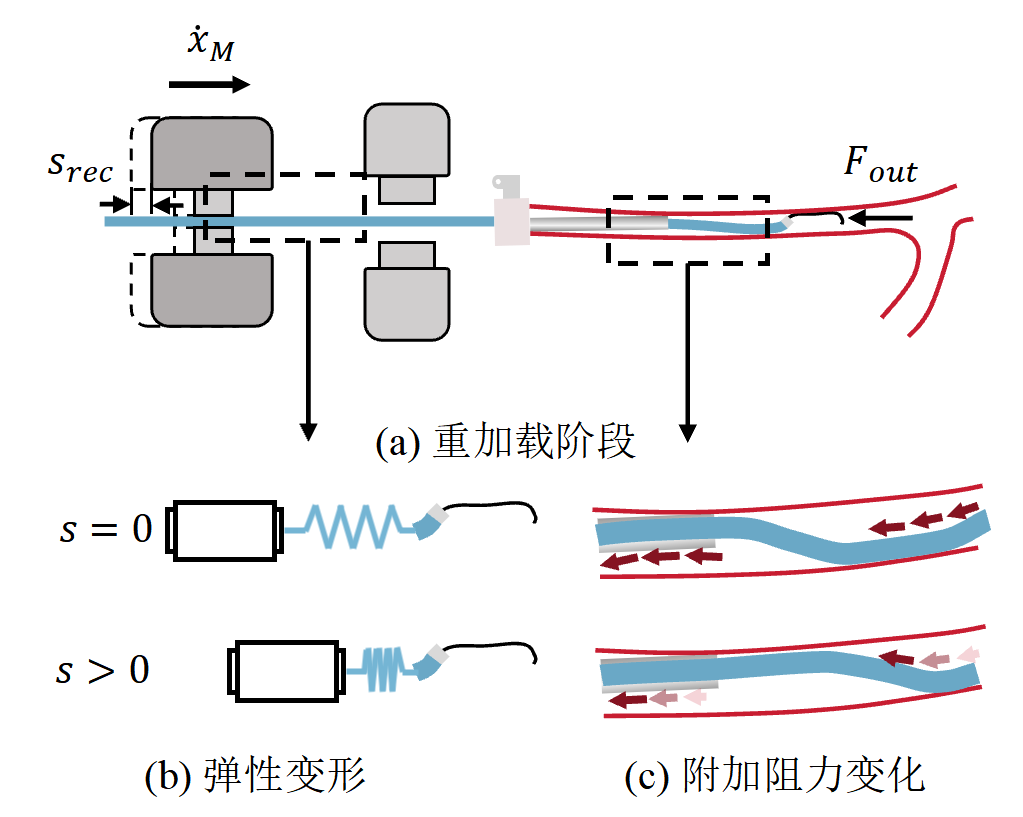
\includegraphics[width=\linewidth]{./figure3_manuscript.png}
\bicaption{轴向载荷恢复与补偿量示意}{Axial load recovery and the compensation term}
\label{fig3}
\end{figure}

\revbegin
切换前载荷 $\widehat D_{9,F}$ 近似代表恢复后的稳态载荷；插入位置变化引起的稳态阻力变化不由恢复模型描述，由2.3节的残差估计网络结合插入深度和前序周期信息修正。
\revend

\subsection{两级残差估计网络与分阶段反馈}

轴向物理模型输出由校正测量值与恢复补偿量组成：
\begin{equation}
\label{eq:physical-model-output}
F_{\mathrm{phys}}[k]=F_{\mathrm{meas}}[k]
+\mathbb I_{\mathrm{rec}}[k]f_{\mathrm{rel},F}(s_{\mathrm{rec}}[k]).
\end{equation}
式中，$\mathbb I_{\mathrm{rec}}=1$ 表示S9中已启用且尚未开始撤除的恢复补偿，其余情况为0。补偿启用时，物理模型输出在恢复起点满足 $F_{\mathrm{phys}}[k_9]=\widehat D_{9,F}$。

残差估计网络用于估计恢复模型未描述的轴向残差。逐点输入为
\begin{equation}
\label{eq:gru-input}
\bm x_k=\big[\widehat D_{9,F},\widehat A_{9,F},t_h,
\bm q_M[k]^{\rm T},s_{\mathrm{rec}}[k],s[k],\sigma[k]\big]^{\rm T}.
\end{equation}
\revbegin
式中，$t_h$ 为S2滑台停止至S9开始的静止时长；$s[k]$ 为插入深度，用于描述随插入位置变化的残差；$\sigma[k]=\operatorname{sgn}\dot x_M[k]$ 为运动方向。$t_h$ 与 $\widehat D_{9,F}$、$\widehat A_{9,F}$ 一样在本次S9开始时确定，网络不使用S9的实时测力值。
\revend

前序周期恢复过程中的运动与承载切换时确定的载荷量可能影响本次恢复时的接触状态，因此采用两级网络引入这些历史信息。第一级在单个恢复过程内按推进行程的先后编码；第二级对前序周期同一行程位置的编码进行加权聚合。

记第 $c$ 个往复周期的S9为第 $c$ 个恢复过程，$c$ 为该周期在试次中的序号。将S9起点之后长度为 $s_{\mathrm{win}}$ 的前向行程等分为 $M$ 个行程单元，第 $m$ 个行程单元的样本集合为
\begin{equation}
\label{eq:phase}
\begin{aligned}
\Omega_{c,m}&=\big\{k\in\mathrm{S9}^{(c)}:(m-1)\Delta s\le s_{\mathrm{rec}}[k]<m\Delta s\big\},\\
\Delta s&=s_{\mathrm{win}}/M,\quad m=1,\cdots,M.
\end{aligned}
\end{equation}
$s_{\mathrm{win}}$ 为统一的恢复补偿行程窗口，依据辨识数据选定，并在训练与测试中固定。该窗口用于确定参考配对区间、网络编码范围和正常推进时的补偿撤除位置。行程单元内无样本时，沿用前一行程单元的特征；首个行程单元无样本时取本周期起点输入。以起点输入初始化GRU，行程单元特征与编码为
\begin{equation}
\label{eq:cell-encoder}
\begin{aligned}
\bm h_{c,0}&=\mathrm{GRU}\big(\bm x_{k_9},\bm 0\big),\\
\bm z_{c,m}&=\frac{1}{|\Omega_{c,m}|}\sum_{k\in\Omega_{c,m}}\bm x_k,\\
\bm h_{c,m}&=\mathrm{GRU}\big(\bm z_{c,m},\bm h_{c,m-1}\big),
\end{aligned}
\end{equation}
式中，$\bm x_{k_9}$ 为本周期S9起点输入，初始化与后续行程单元编码共用同一组GRU参数\ucite{ref26}。$\bm h_{c,m}$ 在 $s_{\mathrm{rec}}$ 到达行程单元终点 $m\Delta s$ 时计算。

% 通栏图4：由最终版 SVG 转为矢量 PDF，按原图175 mm宽度居中排在页顶。
\begin{figure*}[!t]
\centering
\makebox[\textwidth][c]{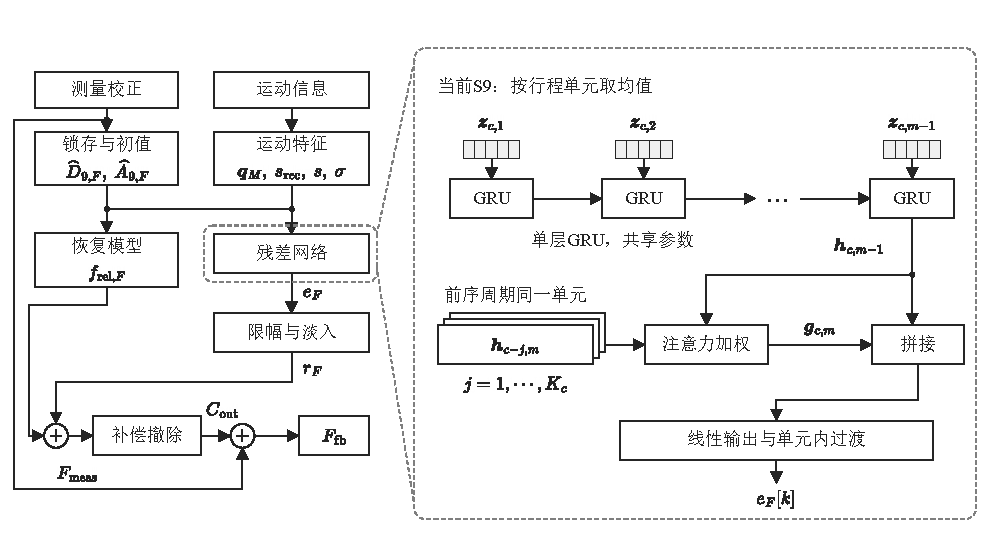
\includegraphics[width=175mm]{./Fig4_最终版.pdf}}
\bicaption{轴向力重构的反馈流程与两级残差估计网络}{Feedback scheme and two-level residual estimation network for axial force reconstruction}
\label{fig4}
\end{figure*}

第二级以当前周期上一行程单元结束时的编码为查询，以此前 $K_c$ 个周期第 $m$ 个行程单元的编码为键和值：
\begin{equation}
\label{eq:cross-cycle}
\begin{aligned}
\bm q_{c,m}&=\bm W_q\bm h_{c,m-1},\\
\bm\kappa_{c,m,j}&=\bm W_k\bm h_{c-j,m},\quad
\bm\upsilon_{c,m,j}=\bm W_v\bm h_{c-j,m},\\
\alpha_{c,m,j}&=\frac{\exp\!\left(\bm q_{c,m}^{\rm T}\bm\kappa_{c,m,j}/\sqrt d\right)}
{\sum_{j'=1}^{K_c}\exp\!\left(\bm q_{c,m}^{\rm T}\bm\kappa_{c,m,j'}/\sqrt d\right)},\\
\bm g_{c,m}&=\sum_{j=1}^{K_c}\alpha_{c,m,j}\bm\upsilon_{c,m,j}.
\end{aligned}
\end{equation}
式中，$K_c=\min(K,c-1)$，$d$ 为编码维度，注意力为单头。$K_c=0$ 时取 $\bm g_{c,m}=\bm 0$，网络只使用当前周期的信息。前序周期第 $m$ 个行程单元的编码在该周期内已经算出，因此第 $m$ 个行程单元的残差估计在进入该行程单元时即可得到：
\begin{equation}
\label{eq:cell-output}
\hat e_{c,m}=\bm w_o^{\rm T}
\begin{bmatrix}\bm h_{c,m-1}\\\bm g_{c,m}\end{bmatrix}+b_o .
\end{equation}
逐点残差在行程单元内由前一行程单元的估计线性过渡到本行程单元的估计：
\begin{equation}
\label{eq:cell-interp}
\begin{aligned}
e_F[k]&=(1-\mu_k)\,\hat e_{c,m-1}+\mu_k\,\hat e_{c,m},\quad k\in\Omega_{c,m},\\
\mu_k&=\frac{s_{\mathrm{rec}}[k]-(m-1)\Delta s}{\Delta s},
\end{aligned}
\end{equation}
式中，$\hat e_{c,0}=0$。残差估计只依赖已经发生的运动，当前周期的运动信息相对输出滞后约一个行程单元长度。达到 $s_{\mathrm{win}}$ 后，按下述规则撤除补偿。

前序周期的编码由运动量和承载切换时确定的载荷量计算，不含S9的实时测力。训练和测试时，每个恢复过程都只使用同一试次中此前已经完成的周期。试次开头的周期没有历史（$K_c=0$），其误差单独统计。残差限幅与残差权重逐步增加规则为
\begin{equation}
\label{eq:residual-limit}
\begin{aligned}
e_{\max,F}&=\eta\widehat A_{9,F}+e_{0,F},\\
r_F[k]&=\beta_k\operatorname{sat}(e_F[k],e_{\max,F}),\\
\beta_k&=\min\!\left\{1,\max\!\left[0,\frac{k-k_9}{N_b}\right]\right\}.
\end{aligned}
\end{equation}
式中，$\operatorname{sat}(e,a)=\max(-a,\min(e,a))$，$\eta\ge0$ 为限幅比例，$e_{0,F}>0$ 为最小限幅，$N_b$ 为残差权重逐步增加所需的采样点数。恢复补偿和残差修正仅在 $\widehat A_{9,F}>0$ 时启用。

正常恢复阶段的总补偿量为 $C[k]=f_{\mathrm{rel},F}(s_{\mathrm{rec}}[k])+r_F[k]$，轴向反馈为
\begin{equation}
\label{eq:active-output}
F_{\mathrm{fb}}[k]=F_{\mathrm{meas}}[k]+C[k].
\end{equation}
补偿启用时 $\beta_{k_9}=0$，故 $F_{\mathrm{fb}}[k_9]=\widehat D_{9,F}$，与切换期间保持的输出衔接。实测值以单位权重进入输出，新增的外部阻力直接反映在反馈中。

当 $s_{\mathrm{rec}}\ge s_{\mathrm{win}}$，或前向速度低于 $v_{\min}$ 持续超过 $T_{\mathrm{st}}$，或出现 $\dot x_M<-v_{\min}$ 的回拉时，开始撤除补偿。记触发时刻为 $t_e$，保存触发前最后一个有效补偿量 $C_e$，随后输出
\begin{equation}
\label{eq:withdrawal}
\begin{aligned}
F_{\mathrm{fb}}[k]&=F_{\mathrm{meas}}[k]+\rho_kC_e,\\
\rho_k&=\max\!\left\{0,1-\frac{t_k-t_e}{T_{\mathrm{off}}}\right\}.
\end{aligned}
\end{equation}
式中，$v_{\min}$ 为最小有效前向速度，$T_{\mathrm{st}}$ 为停止判定时长，$T_{\mathrm{off}}$ 为补偿撤除时长。撤除期间恢复模型与残差估计网络的输出不再更新；$\rho_k=0$ 后只输出校正测量值。因停止或回拉而退出时，本次恢复补偿不再重新启用。正常推进达到窗口终点并撤除补偿后进入S10。

令 $C_{\mathrm{out}}[k]$ 在正常恢复时为 $C[k]$，撤除时为 $\rho_kC_e$，未启用或已撤除时为0。全周期反馈为
\begin{equation}
\label{eq:phase-output}
\bm w_{\mathrm{fb}}[k]=
\begin{cases}
\widehat{\bm D}_9,&k\in\mathrm{S2}\sim\mathrm{S8},\\
\begin{bmatrix}F_{\mathrm{meas}}[k]+C_{\mathrm{out}}[k]\\
\tau_{\mathrm{meas}}[k]\end{bmatrix},&k\in\mathrm{S9},\\
\bm w_{\mathrm{meas}}[k],&k\in\{\mathrm{S1},\mathrm{S10}\}.
\end{cases}
\end{equation}
当 $\widehat A_{9,F}\le0$ 时，S9的 $C_{\mathrm{out}}=0$。扭矩在S9直接输出校正测量值。

网络训练采用与在线计算一致的限幅和残差权重逐步增加规则。令 $\Omega_{\mathrm{S9}}$ 为训练集中具有配对参考、且启用正常恢复补偿的S9样本，$\mathcal P_{\mathrm{S9}}$ 为同一恢复过程内、均属于 $\Omega_{\mathrm{S9}}$ 且时间相邻的样本对，损失函数为
\begin{equation}
\label{eq:gru-loss}
\begin{aligned}
\mathcal L={}&\frac{1}{|\Omega_{\mathrm{S9}}|}\sum_{k\in\Omega_{\mathrm{S9}}}
\left(\frac{F_{\mathrm{ref}}(s[k])-F_{\mathrm{phys}}[k]-r_F[k]}{F_*}\right)^2\\
&+\frac{\gamma_{\mathrm{sm}}}{|\mathcal P_{\mathrm{S9}}|}
\sum_{(j,k)\in\mathcal P_{\mathrm{S9}}}
\left(\frac{r_F[k]-r_F[j]}{F_*}\right)^2.
\end{aligned}
\end{equation}
\revbegin
式中，$F_{\mathrm{ref}}$ 按式\eqref{eq:reference}取自配对连续递送参考，$F_*>0$ 为由训练集确定的力归一化尺度，$\gamma_{\mathrm{sm}}$ 为平滑权重。连续递送参考与往复递送的配对记录作为同一组划分至训练、验证或测试集，输入标准化参数仅由训练集计算。方法流程如图\ref{fig4}所示。
\revend



\section{实验验证与分析（Experimental validation and analysis）}

\revbegin
\subsection{实验平台与实验配置}
\revend

\revbegin
实验平台采用自主研制的血管介入机器人，介入器械包括0.014英寸导引导丝与6F介入导管。递送机构滑台的平移与旋转由伺服电机驱动。近端测力机构采用两只力恒LH-S09A3单轴拉压传感器，分别测量轴向力和切向力；切向力经标定等效力臂换算为扭矩。测量与控制系统基于倍福控制总线构建，以 $250\,{\rm Hz}$ 同步记录测力读数、各轴位置、速度、加速度及夹持组件开合指令。
\revend

\revbegin
测量参数标定时，将测力单元与外部标准力传感器串联，施加已知轴向载荷及已知力臂的切向载荷，标定传递矩阵 $\bm H_0$ 和传感器等效力臂 $\ell_s$，并通过空载角度扫描辨识空载响应项。标定参数及残差统计为[待补]。连续递送参考由递送机构持续夹持器械采集，鞘管、血管模型路径和起始插入位置与往复递送试次匹配，参考区间按实际插入位置及运动条件配对。图\ref{fig5}展示测力单元标定与递送平台，外接标准力传感器用于标定，血管模型构成器械递送路径。
\revend

\begin{figure}[!htbp]
\centering
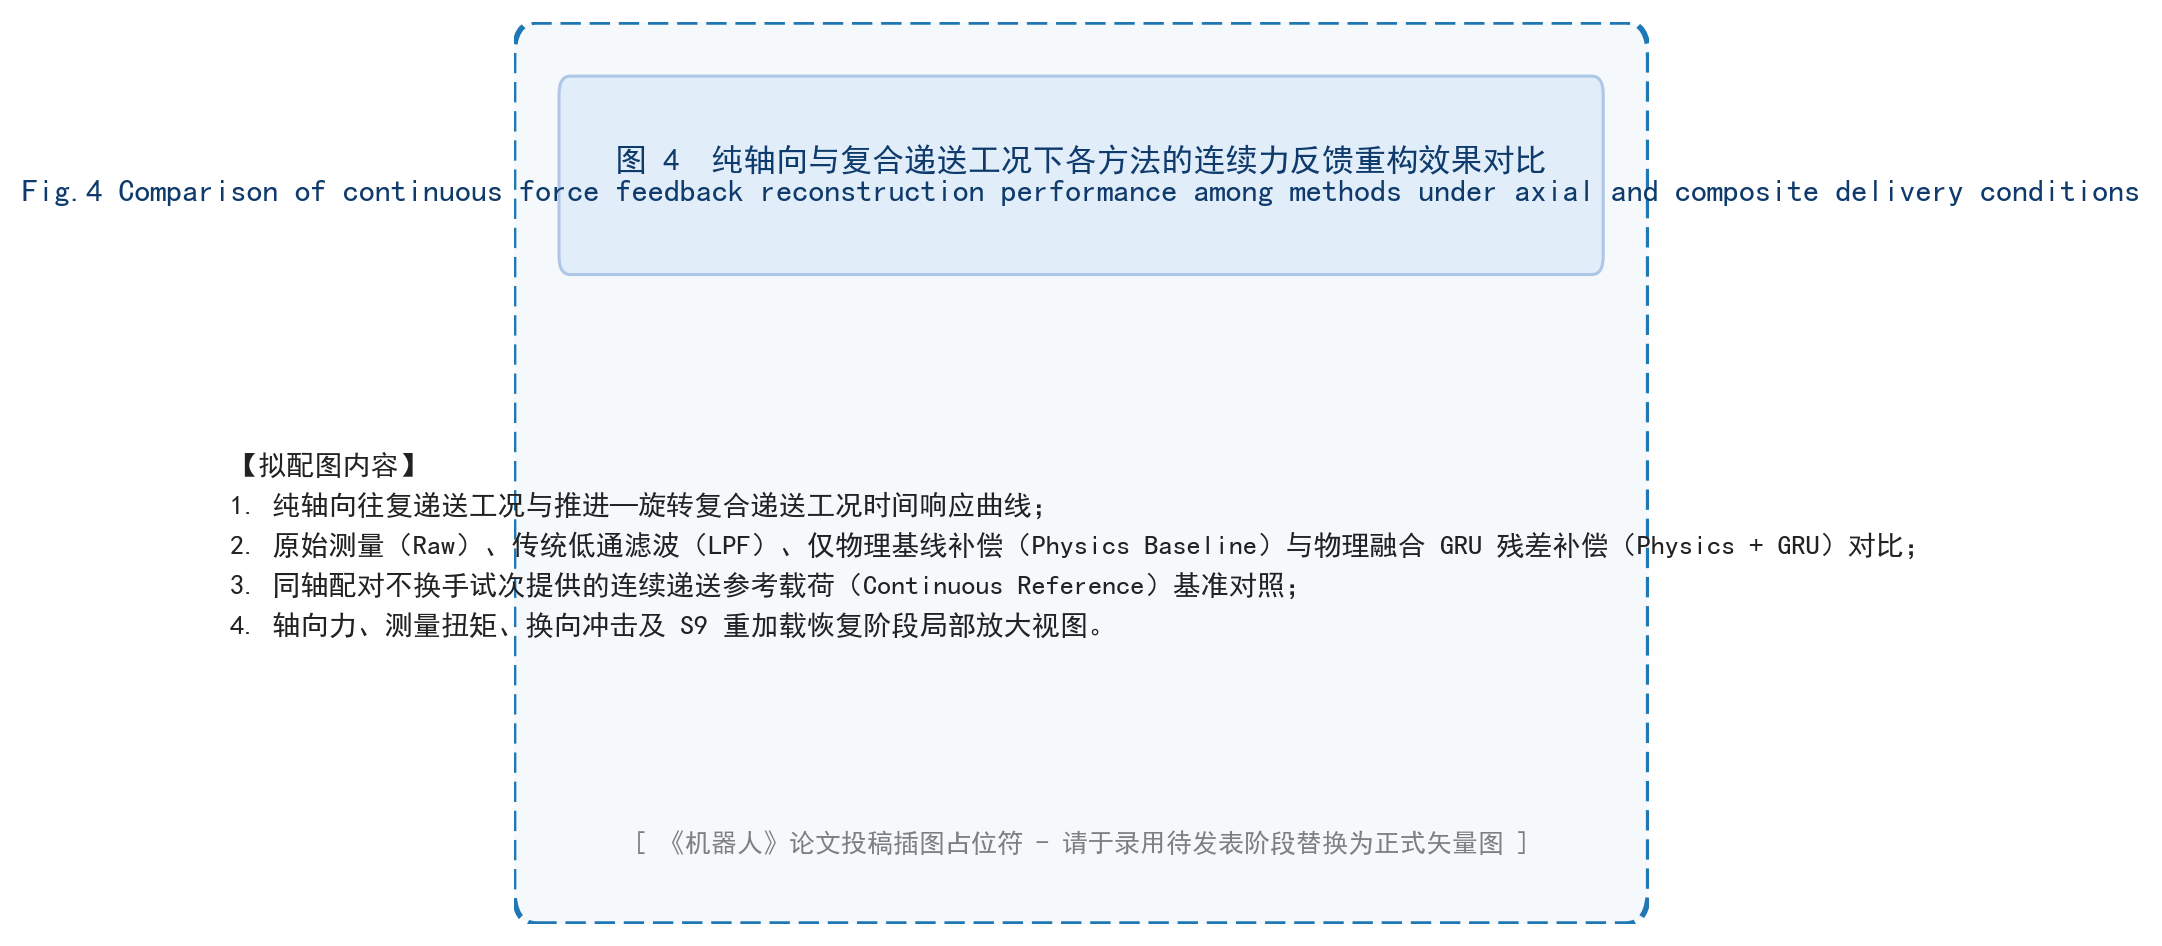
\includegraphics[width=\linewidth]{fig4.png}
\bicaption{\revised{测量参数标定与往复递送实验设置}}{\revised{Experimental configurations for measurement calibration and reciprocating delivery}}
\label{fig5}
\end{figure}

\revbegin
所有往复递送试次均在器械经导管鞘进入血管模型的同一装置中完成。推进速度设多档，指令值为 $7$～$60\,\mathrm{mm/s}$，各速度档S1与S9采用相同速度指令。各周期静止时长约为 $1.9$～$4.1\,\mathrm{s}$，插入深度随周期增加。连续递送参考的单次行程不超过 $20\,\mathrm{mm}$，覆盖统一恢复窗口 $s_{\mathrm{win}}$ 及相邻递送段；配对试次数、运动条件和重复次数为[待补]。
\revend

\revbegin
\subsection{载荷转移与恢复模型辨识}
\revend

\revbegin
在承载切换过程中比较递送机构与支撑机构的载荷变化，S4和S8分别对应测力通道卸载与重新承载。S8末递送机构载荷增量与S7末支撑机构载荷之比约为0.74，统计结果为[待补]。S8末仍存在待恢复载荷差。
\revend

\revbegin
以完整恢复模型为主，自 $s_{\mathrm{rec}}=0.77\,\mathrm{mm}$ 起拟合（起点选择原因为[待补]），比较附加摩擦阻力项和弹性加载项的作用。外部留出集共15个文件、113个周期，其中87个周期出现局部峰值，判据为窗口内最大值相对 $\widehat D_{9,F}$ 和末段载荷中位数的峰值超出量均至少为 $0.05\,\mathrm{N}$。不计附加摩擦阻力时，仅弹性加载模型无法给出局部峰值，相对实测恢复曲线的整窗均方根误差（RMSE）由 $0.412\,\mathrm{N}$ 升至 $0.480\,\mathrm{N}$，前 $1\,\mathrm{mm}$ 的RMSE由 $0.534\,\mathrm{N}$ 升至 $0.658\,\mathrm{N}$；完整恢复模型正确识别出其中70个局部峰值。不计弹性加载时，仅附加摩擦（$\lambda_F\to0$）的误差为[待补]，补偿输出在S9起始出现与待恢复载荷差相当的凹陷。校正测量及三种模型形式相对参考的S9误差分布见图\ref{fig6}(b)，辨识参数 $\lambda_F$、$\Delta_F$、$D_c$ 及峰位误差为[待补]。
\revend

\revbegin
恢复窗口末端载荷与切换前载荷的绝对偏差中位数约为 $0.2\,\mathrm{N}$，这部分由残差估计网络处理。
\revend

\revbegin
\begin{figure}[H]
\centering
\fbox{\parbox{0.92\linewidth}{\raggedright [待补]\par
(a) 典型周期实测S9载荷、仅弹性加载与完整恢复模型曲线，以及补偿后输出；\par
(b) 外部留出集上校正测量、仅附加摩擦、仅弹性加载与完整恢复模型的S9误差箱线图。}}
\bicaption{\revised{轴向载荷恢复模型辨识结果}}{\revised{Identification results of the axial load recovery model}}
\label{fig6}
\end{figure}
\revend

\revbegin
\subsection{力反馈性能评价}
\revend

\revbegin
数据按完整试次划分，连续递送参考与对应往复试次置于同一数据组，验证集用于选择超参数，外部留出集用于报告结果。测试前冻结物理参数、网络参数及标准化参数，网络采用 $M=20$ 个行程单元、$K=10$ 个历史周期和维度 $d=32$ 的单层GRU编码器与单头跨周期注意力。比较方法包括校正测量值直接输出、保持至S8（S2～S8保持切换前载荷，S9起输出校正测量值）、恢复模型补偿（仅弹性加载）、恢复模型补偿、恢复模型+单周期GRU、本文方法（恢复模型+跨周期注意力残差网络）和不含恢复模型的纯网络。训练与验证试次数及优化设置为[待补]，多周期轴向反馈波形及一次S9恢复反馈误差见图\ref{fig9}。
\revend

\revbegin
\begin{figure}[H]
\centering
\fbox{\parbox{0.92\linewidth}{\raggedright [待补]\par
(a) 多周期反馈波形，两机构交替承载期间的输出保持段截断显示；\par
(b) 一次S9恢复的反馈误差，对比保持至S8、保持至S9、恢复模型补偿与本文方法。}}
\bicaption{\revised{血管模型中的多周期轴向反馈重构}}{\revised{Axial force feedback reconstruction over multiple cycles in a vascular phantom}}
\label{fig9}
\end{figure}
\revend

\subsubsection{参考误差分析}

\revbegin
S9 RMSE和S9前 $1\,\mathrm{mm}$ RMSE分别为相应区间内反馈相对参考载荷的均方根误差，S2～S10误差峰峰值为该区间内反馈误差的最大值与最小值之差。S1和S10阶段各方法均输出校正测量值，其误差为[待补]。外部留出集上七种方法的轴向误差汇总于表\ref{tab1}，差异统计为[待补]。
\revend

\revbegin
\begin{table*}[t]
\RevisionColor
\centering
\bicaption{\revised{外部留出集上的轴向力反馈误差}}{\revised{Axial force feedback errors on the external held-out set}}
\label{tab1}
\small
\setlength{\tabcolsep}{5pt}
\begin{tabular}{p{0.40\textwidth}ccc}
\toprule
对比方法 & \shortstack{S9 RMSE\\(N)} & \shortstack{S9前1 mm\\RMSE (N)} & \shortstack{S2～S10误差\\峰峰值 (N)}\\
\midrule
校正测量值直接输出 & [待补] & [待补] & [待补]\\
保持至S8 & [待补] & [待补] & [待补]\\
恢复模型补偿（仅弹性加载） & [待补] & [待补] & [待补]\\
恢复模型补偿 & [待补] & [待补] & [待补]\\
恢复模型+单周期GRU & [待补] & [待补] & [待补]\\
本文方法（恢复模型+跨周期注意力残差网络） & [待补] & [待补] & [待补]\\
不含恢复模型的纯网络 & [待补] & [待补] & [待补]\\
\bottomrule
\end{tabular}
\end{table*}
\revend

\revbegin
\subsubsection{叠加阻力响应评估}
\revend

\revbegin
从外部留出集随机选取若干S9周期（周期数为[待补]），在校正测量值与参考载荷上同时叠加设定幅值的阶跃阻力和短时脉冲阻力，按各方法重新计算反馈输出，幅值、施加位置和脉冲宽度为[待补]。反馈增量取叠加前后输出之差，阶跃保留比为反馈增量平台均值与叠加幅值之比，响应延迟为反馈增量与参考增量达到叠加幅值63\%的时间差，脉冲保留比为反馈增量峰值与脉冲幅值之比。保持至S9在S9内对叠加阻力无响应，直至S10才出现；保持至S8能够保留叠加阻力，但反馈带有恢复凹陷。恢复模型补偿与本文方法的补偿量均不使用S9实时测力，叠加阻力以单位权重进入反馈，两者响应相同；阶跃与脉冲保留比及响应延迟为[待补]。低速周期在S9中叠加阶跃阻力时各方法的反馈见图\ref{fig7}。
\revend

\revbegin
\begin{figure}[H]
\centering
\fbox{\parbox{0.92\linewidth}{\raggedright [待补]\par
(a) 低速周期在S9中叠加阶跃阻力时各方法的反馈。}}
\bicaption{\revised{S9阶段叠加阻力的反馈响应}}{\revised{Feedback responses to superimposed resistance during S9}}
\label{fig7}
\end{figure}
\revend

\revbegin
\subsection{操作者实验}
\revend

\revbegin
操作者实验采用缩短后的往复夹持时序，比较未校正反馈与本文方法两种条件；每名操作者每种条件完成2组，按ABBA平衡顺序进行，操作者不知晓当前条件，人数为[待补]。评价指标包括介入总时间、通过成功率、总推进行程与路径长度之比及回撤次数；两机构交替承载期间的输出跌落幅值、承载机构切换瞬间的输出跳变量和S2～S10输出峰峰值用于评价反馈连续性，均由反馈输出计算，无需连续递送参考。各项实验结果为[待补]，见图\ref{fig10}。
\revend

\revbegin
\begin{figure}[H]
\centering
\fbox{\parbox{0.92\linewidth}{\raggedright [待补]\par
(a) 两种反馈条件下的介入总时间、通过成功率、总推进行程与路径长度之比及回撤次数；\par
(b) 两机构交替承载期间的输出跌落幅值、承载机构切换瞬间的输出跳变量和S2～S10输出峰峰值。标明操作者人数、试次数和统计量。}}
\bicaption{\revised{不同轴向反馈条件下的操作者任务表现}}{\revised{Operator task performance under different axial force-feedback conditions}}
\label{fig10}
\end{figure}
\revend

\section{讨论（Discussion）}

\revbegin
传力链弹性加载和停顿后附加摩擦阻力衰减分别对应起步段加载与局部峰值。计入附加摩擦阻力后，恢复模型能够描述局部峰值和起步段载荷变化。恢复窗口末端约 $0.2\,\mathrm{N}$ 的稳态偏差及周期间差异由残差估计网络修正，消融结果为[待补]。叠加阻力测试表明，补偿量与实时测力解耦，使S9阶段新增阻力不被补偿削弱。
\revend

\revbegin
按行程单元编码使不同速度下的恢复过程具有一致的表示长度，并可按行程位置对齐前序周期。跨周期聚合对残差估计的贡献见表\ref{tab1}，结果为[待补]。
\revend

\revbegin
本文静止时长范围较窄，附加阻力幅值与静止时长的关系、初始加载刚度与插入深度的关系均未辨识。模型结构与Dahl预滑动及速率--状态摩擦的形式一致\cite{dahl1968,ruina1983}，可通过不发生夹持状态切换的停--走试验进一步辨识。叠加阻力测试为离线叠加，实际阻力突变对接触状态的影响需结合实物加载评价。
\revend

\section{结论（Conclusions）}

\revbegin
本文建立了结合空载响应项校正、载荷转移分析、轴向载荷恢复模型和跨周期残差估计网络的力反馈重构方法。恢复模型以传力链弹性加载与停顿后附加摩擦阻力衰减描述S9的载荷变化，三个参数离线联合辨识后冻结。GRU和跨周期注意力估计恢复模型未描述的残差，结合切换期间的输出保持与补偿量平滑撤除，形成分阶段反馈。补偿量与S9实时测力解耦，离线叠加阻力可完整进入反馈；反馈重构误差及操作者实验的定量结果为[待补]。
\revend

\noindent

% -------- 参考文献表
\bibliographystyle{JQR_LaTeX_Template-0507/jqr-num}
\bibliography{JQR_LaTeX_Template-0507/references}

\begin{AuthorIntroduction}
\Intro 第一作者：隋凯丞（2000--），男，硕士研究生。研究领域：血管介入手术机器人，机器人力感知与控制。E-mail: suikaicheng24@mails.ucas.ac.cn。
\revbegin

\Intro
通信作者：胡琨元（出生年份[待补]），作者简介与E-mail为[待补]。
\revend

\Intro 通信作者：刘浩（1976--），男，博士，研究员，博士生导师。研究领域：医疗微创手术机器人，智能控制。E-mail: liuhao@sia.cn。

\end{AuthorIntroduction}

\balance
\end{document}
